\documentclass[letterpaper,11pt,oneside,reqno]{article}

%%%%%%%%%%%%%%%%%%%%%%%%%%%%%%%%%%%%%%%%%%%%%%%%%%%%%%%%%%%%

\usepackage[pdftex,backref=page,colorlinks=true,linkcolor=blue,citecolor=red]{hyperref}
\usepackage[alphabetic,nobysame]{amsrefs}

%%%%%%%%%%%%%%%%%%%%%%%%%%%%%%%%%%%%%%%%%%%%%%%%%%%%%%%%%%%%
%main packages
\usepackage{amsmath,amssymb,amsthm,amsfonts,mathtools}
\usepackage{graphicx,color}
\usepackage{upgreek}
\usepackage[mathscr]{euscript}

%equations
\allowdisplaybreaks
\numberwithin{equation}{section}

%tikz
\usepackage{tikz}
\usetikzlibrary{shapes,arrows,positioning,decorations.markings}

%conveniences
\usepackage{array}
\usepackage{adjustbox}
\usepackage{cleveref}
\usepackage{enumerate}
\usepackage{datetime}
\usepackage{comment}

%paper geometry
\usepackage[DIV=12]{typearea}

%%%%%%%%%%%%%%%%%%%%%%%%%%%%%%%%%%%%%%%%%%%%%%%%%%%%%%%%%%%%
%draft-specific
\synctex=1
% \usepackage{refcheck,comment}

%%%%%%%%%%%%%%%%%%%%%%%%%%%%%%%%%%%%%%%%%%%%%%%%%%%%%%%%%%%%
%this paper specific
\newcommand{\ssp}{\hspace{1pt}}

%%%%%%%%%%%%%%%%%%%%%%%%%%%%%%%%%%%%%%%%%%%%%%%%%%%%%%%%%%%%
\newtheorem{proposition}{Proposition}[section]
\newtheorem{lemma}[proposition]{Lemma}
\newtheorem{corollary}[proposition]{Corollary}
\newtheorem{theorem}[proposition]{Theorem}
%%%%%%%%%%%%%%%%%%%%%%%%%%%%%%%%%%%%%%%%%%%%%%%%%%%%%%%%%%%%
\theoremstyle{definition}
\newtheorem{definition}[proposition]{Definition}
\newtheorem{remark}[proposition]{Remark}
\newtheorem{example}[proposition]{Example}
%%%%%%%%%%%%%%%%%%%%%%%%%%%%%%%%%%%%%%%%%%%%%%%%%%%%%%%%%%%%


\newenvironment{lnotes}{\section*{Notes for the lecturer}}{}
% \excludecomment{lnotes}


\begin{document}
\title{Lectures on Random Matrices
(Spring 2025)
\\Lecture 4: Semicircle law via tridiagonalization. \\Orthogonal polynomial ensembles}


\date{Wednesday, January 29, 2025\footnote{\href{https://lpetrov.cc/rmt25/}{\texttt{Course webpage}}
$\bullet$ \href{https://lpetrov.cc/rmt25/rmt25-notes/rmt2025-l04.tex}{\texttt{TeX Source}}
$\bullet$
Updated at \currenttime, \today}}



\author{Leonid Petrov}


\maketitle
\tableofcontents

\section{Recap}

Note: I did some live random matrix simulations
\href{https://lpetrov.cc/simulations/2025-01-28-goe/}{here}
and
\href{https://lpetrov.cc/simulations/2025-01-28-bbp-transition/}{here}
--- check them out. More simulations to come.

\subsection{Gaussian ensembles}

We introduced Gaussian ensembles,
and for GOE ($\beta=1$) we computed the joint eigenvalue density.
The normalization is so that the off-diagonal elements have variance $\frac{1}{2}$
and the diagonal elements have variance $1$.
Then the joint eigenvalue density is
\begin{equation*}
	p(\lambda_1,\ldots,\lambda_n)
	=
	\frac{1}{Z_n}\,
	\prod_{i=1}^n e^{-\frac{1}{2}\lambda_i^2}
	\prod_{1\le i<j\le n}(\lambda_i - \lambda_j),
	\qquad
	\lambda_1\ge \lambda_2\ge \ldots \ge \lambda_n.
\end{equation*}

\subsection{Tridiagonalization}

We showed that any real symmetric matrix \(A\) can be tridiagonalized by an orthogonal transformation \(Q\):
\[
	Q^\top\,A\,Q \;=\; T,
\]
where \(T\) is real symmetric tridiagonal, having nonzero entries only on the main diagonal and the first super-/subdiagonals:
\begin{equation*}
	T \;=\;
	\begin{pmatrix}
		 d_1 & \alpha_1 & 0 & \cdots & 0\\
		 \alpha_1 & d_2 & \alpha_2 & \cdots & 0\\
		 0 & \alpha_2 & d_3 & \ddots & \vdots\\
		 \vdots & \vdots & \ddots & \ddots & \alpha_{n-1}\\
		 0 & 0 & \cdots & \alpha_{n-1} & d_n
	\end{pmatrix}.
\end{equation*}
In the proof, each time we need to act in the orthogonal complement to the
subspace $e_1,\ldots,e_{k-1}$ (starting from $e_1$),
and apply a Householder reflection to zero out everything strictly
below the subdiagonal. (We apply the transformations like
$A\mapsto H A H^{\top}$, so that the first row transforms
in the same way as the first column of $A$).

\section{Tridiagonal random matrices}

\subsection{Distribution of the tridiagonal form of the GOE}

Applying the tridiagonalization to GOE, we obtain the following
random matrix model.

\begin{theorem}
\label{thm:DE-model}
Let \(W\) be an \(n\times n\) GOE matrix (real symmetric) with variances chosen so that each off-diagonal entry has variance \(1/2\) and each diagonal entry has variance \(1\).  Then there exists an orthogonal matrix \(Q\) such that
\[
   W \;=\; Q^\top\,T\,Q,
\]
where \(T\) is a real symmetric tridiagonal matrix
\begin{equation}
	\label{eq:tridiagonal-form}
   T \;=\; \begin{pmatrix}
         d_1 & \alpha_1 & 0 & \cdots \\
         \alpha_1 & d_2 & \alpha_2 & \ddots \\
         0 & \alpha_2 & d_3 & \ddots \\
         \vdots & \ddots & \ddots & \ddots
       \end{pmatrix},
\end{equation}
and the random variables \(\{d_i,\alpha_j\}_{1 \le i \le n,\;1\le j\le n-1}\) are mutually independent, with
\[
  d_i \,\sim\, \mathcal{N}(0,1),
  \qquad
  \alpha_j \;=\; \sqrt{\frac{\chi^2_{\,n-j}}{2}},
\]
where \(\chi^2_{\nu}\) is a chi-square distribution with \(\nu\) degrees of freedom.
\end{theorem}

\begin{remark}[Chi-square distributions]
The \emph{chi-square distribution} with \(\nu\) degrees of
freedom, denoted by \(\chi^2_{\nu}\), is a fundamental
distribution in statistics and probability theory. It arises
naturally as the distribution of the sum of the squares of
\(\nu\) independent standard normal random variables.
Formally, if \(Z_1, Z_2, \ldots, Z_{\nu}\) are independent
random variables with \(Z_i \sim \mathcal{N}(0,1)\), then
the random variable
\[
  Q = \sum_{i=1}^{\nu} Z_i^2
\]
follows a chi-square distribution with \(\nu\) degrees of
freedom, i.e., \(Q \sim \chi^2_{\nu}\). In the context of
\Cref{thm:DE-model}, the $\alpha_j$'s can be called \emph{chi random variables}.

The parameter $\nu$ does not need to be an integer, and the
chi-square distribution is well defined for any positive
real $\nu$, for example, by continuation of the density formula.
The probability density is
\begin{equation*}
	f(x) \;=\; \frac{1}{2^{\nu/2}\,\Gamma(\nu/2)}\,x^{\nu/2-1}\,e^{-x/2},
	\qquad x\ge 0.
\end{equation*}
\end{remark}

\begin{proof}[Proof of \Cref{thm:DE-model}]
	In the process of tridiagonalization,
	we apply Householder reflections.
	Note that the diagonal entries stay fixed,
	and we only change the off-diagonal entries.
	Let us consider these off-diagonal entries.

	In the first step, we apply the reflection in $\mathbb{R}^{n-1}$
	to turn the column vector $(a_{2,1},a_{3,1},\ldots,a_{n,1} )$ into
	a vector parallel to $(1,0,\ldots,0)\in \mathbb{R}^{n-1}$.
	Since the Householder reflection is orthogonal,
	it preserves lengths. So,
	\begin{equation*}
		\alpha_1=\sqrt{a_{21}^2+a_{31}^2+\cdots+a_{n1}^2},\qquad a_{i1}\sim
		\mathcal{N}(0,\dfrac{1}{2}).
	\end{equation*}
	This implies that $\alpha_1$ has the desired chi distribution.
	The distribution of the other entries is obtained similarly by the recursive
	application of the Householder reflections.

	Note that $\alpha_j$'s and $d_i$'s depend on nonintersecting
	subsets of the matrix entries, so they are independent. This completes the proof.
\end{proof}



\subsection{Dumitriu--Edelman G$\beta$E tridiagonal random matrices}

Let us define a general $\beta$ extension of the tridiagonal model for the
GOE.

\begin{definition}
	\label{def:tridiagonal-model-general-beta}
	Let $\beta>0$ be a parameter.
	The tridiagonal G$\beta$E is a random $n\times n$
	tridiagonal real symmetric
	matrix $T$ as in
	\eqref{eq:tridiagonal-form},
	where $d_i\sim \mathcal{N}(0,1)$ are independent standard Gaussians,
	and
	\begin{equation*}
		\alpha_j\sim \frac{1}{\sqrt 2}\chi_{\beta(n-j)},\qquad
		1\le j\le n-1,
	\end{equation*}
	are chi-distributed random variables.
\end{definition}

We showed that for $\beta=1$,
the G$\beta$E is the tridiagonal form of the GOE random matrix model.
The same holds for the two other classical betas:
\begin{proposition}[Without proof]
	\label{prop:tridiagonal-model-beta-classical}
	For $\beta=2$, the G$\beta$E is the tridiagonal form of the GUE random matrix model,
	which is the random complex Hermitian matrix with Gaussian entries and maximal
	independence. Similarly, for $\beta=4$,
	the G$\beta$E is the tridiagonal form of the GSE random matrix model.
\end{proposition}


Moreover, for all $\beta$, the joint eigenvalue density of G$\beta$E is
explicit:
\begin{theorem}[\cite{dumitriu2002matrix}]
	\label{thm:DE-joint-eigenvalue-density}
	Let \(T\) be a G$\beta$E matrix as in \Cref{def:tridiagonal-model-general-beta}.
	Then the joint eigenvalue density is given by
	\begin{equation*}
		p(\lambda_1,\ldots,\lambda_n)
		=
		\frac{1}{Z_{n,\beta}}\,
		e^{-\frac{1}{2}\sum_{i=1}^n \lambda_i^2}
		\prod_{1\le i<j\le n}|\lambda_i - \lambda_j|^\beta,
		\qquad
		\lambda_1\ge \lambda_2\ge \ldots \ge \lambda_n.
	\end{equation*}
\end{theorem}

This theorem is also given without proof. The proof involves
linear algebra and computation of the Jacobians of the
change of variables from the matrix entries to the
eigenvalues in the tridiagonal setting.  It can be found in
the original paper \cite{dumitriu2002matrix}.

\subsection{The case \texorpdfstring{$\beta=2$}{beta=2}}
\label{subsec:beta2-case}

For many questions involving \emph{local eigenvalue statistics},
the case \(\beta=2\) (the GUE, Gaussian Unitary Ensemble) is the most tractable.
This is because the joint density of the eigenvalues
admits a determinantal structure coming from
a \emph{square} Vandermonde factor
\(\,\prod_{i<j} (\lambda_i - \lambda_j)^2\)
and the Gaussian exponential
\(\,\exp\bigl(-\tfrac12 \sum \lambda_j^2\bigr)\).
Moreover, for \(\beta=2\), the random matrix model
and its correlation functions
can be expressed explicitly through determinants involving
\emph{orthogonal polynomials}, namely, the \emph{Hermite polynomials}.

\begin{proposition}[Joint density for GUE and orthogonal polynomials]
  \label{prop:gue-joint-density}
  Consider the GUE (Gaussian Unitary Ensemble) random matrix model, i.e.\ an
  \(n\times n\) complex Hermitian matrix whose entries
  are i.i.d.\ up to the Hermitian condition, with each
  off-diagonal entry distributed as
  \(\mathcal{N}(0,\tfrac12)+\mathrm{i}\,\mathcal{N}(0,\tfrac12)\)
  and each diagonal entry \(\mathcal{N}(0,1)\).
  The ordered eigenvalues \(\lambda_1 \ge \cdots \ge \lambda_n\)
  (or, without ordering, thought of as an unordered set)
  satisfy the joint probability density
  \begin{equation}
  	\label{eq:gue-joint-density}
    p(\lambda_1,\ldots,\lambda_n)
    \;=\;
    \frac{1}{Z_{n,2}}
    \prod_{j=1}^n e^{-\frac12 \lambda_j^2}
    \;\prod_{1\le i<j\le n} (\lambda_i - \lambda_j)^2,
  \end{equation}
  where \(Z_{n,2}\) is a normalization constant.

	Moreover, if
  \(\{\psi_k(\lambda)\}_{k=0}^\infty\)
	is the family of Hermite polynomials, orthonormal
  with respect to the measure
  \(w(\lambda)\,d\lambda = e^{-\lambda^2/2}\,d\lambda\)
  on \(\mathbb{R}\) (i.e.,
	\(\displaystyle\int_{-\infty}^{\infty} \psi_k(\lambda)\,\psi_\ell(\lambda)\,w(\lambda)\,d\lambda = \mathbf{1}_{k=\ell}\)),
  then one can also write
  \begin{equation}
  	\label{eq:gue-joint-OP}
    p(\lambda_1,\ldots,\lambda_n)
    \;=\;
		\mathrm{const}\cdot
		\det\Bigl[\psi_{j-1}(\lambda_k)e^{-\frac{\lambda_k^2}{4}}\Bigr]_{j,k=1}^n
		\;\det\Bigl[\psi_{j-1}(\lambda_k)e^{-\frac{\lambda_k^2}{4}}\Bigr]_{j,k=1}^n
  \end{equation}
	(the two determinants are identical, but let us keep this notation for future convenience).
\end{proposition}
The \emph{square determinant} structure is extremely useful.
It is
precisely the \(\beta=2\) counterpart
of the squared Vandermonde factor
\(\,\prod_{i<j}(\lambda_i-\lambda_j)^2\).


\begin{remark}[Hermite polynomials]
  There are various normalizations of Hermite polynomials.
  In random matrix theory for the Gaussian ensembles,
  we often use the \emph{probabilists' Hermite polynomials}
	(sometimes called \(\mathrm{He}_k\), but we use the notation $H_k$).
	There are various normalizations due to the factor in the exponent
	of $x^2$.

  A convenient definition for use with the weight \(e^{-x^2/2}\) is:
  \[
    H_k(x)
    \;=\;
    (-1)^k\, e^{\tfrac{x^2}{2}}
    \frac{d^k}{dx^k}
    \Bigl(e^{-\tfrac{x^2}{2}}\Bigr),
		\qquad
		k=0,1,\ldots,
  \]
  whose leading term is \(x^k\).
	Polynomials with the leading coeffient \(1\) are called \emph{monic}.
	The first few monic Hermite polynomials are
	\[
		H_0(x) = 1,\qquad
		H_1(x) = x,\qquad
		H_2(x) = x^2 - 1,\qquad
		H_3(x) = x^3 - 3x,\qquad
		H_4(x) = x^4 - 6x^2 + 3.
	\]
	The difference between $H_k$ and $\psi_k$ entering \Cref{prop:gue-joint-density}
	is in a constant normalization,
	since $H_k$ are monic but not orthonormal,
	while $\psi_k$ are orthonormal but not monic.
\end{remark}

\begin{proof}[Sketch of the determinantal representation]
  In brief, one observes that the factor
  \(\prod_{i<j}(\lambda_i - \lambda_j)\)
  is exactly the Vandermonde determinant
  \(\Delta(\lambda_1,\dots,\lambda_n)
  = \det\bigl[\lambda_k^{j-1}\bigr]_{j,k=1}^n\).
	Next, the Vandermonde determinant is also equal to
	the determinant built out of any monic family of polynomials of the corresponding
	degrees (by linear transformations), and so we get the desired
	representation.
\end{proof}

We will work with Hermite polynomials
and the determinantal structure in \Cref{prop:gue-joint-density}
in the next
\href{https://lpetrov.cc/rmt25/rmt25-notes/rmt2025-l05.pdf}{Lecture 5}).

\section{Wigner semicircle law via tridiagonalization}
\label{sec:semicircle-tridiagonal}


If $W$ is an $n\times n$ real Wigner matrix with entries of
mean zero and variance $1$ on the off-diagonal, then as
$n\to\infty$, the empirical spectral distribution (ESD) of
$W/\sqrt{n}$ converges weakly almost surely to the Wigner
semicircle distribution:
\[
  \mu_{\mathrm{sc}}(dx)
  \;=\;
  \frac{1}{2\pi}\,\sqrt{4 - x^2}\,\mathbf{1}_{|x|\le2}\,dx.
\]
We already derived this in
\href{https://lpetrov.cc/rmt25/rmt25-notes/rmt2025-l02.pdf}{Lecture 2}
by a direct combinatorial argument on the trace. Now we present another proof by using the tridiagonal form of $W$.  The argument is conceptually simpler in some steps, because the matrix is sparser (only tridiagonal).
At the same time, we will establish the Wigner
semicircle law for the general G$\beta$E case (but only Gaussian), and
thus it will apply to GUE and GSE.

%%%%%%%%%%%%%%%%%%%%%%%%%%%%%%%%%%%%%%%%%%%%%%%%%%%%%%%%%%%%
\subsection{Moments for tridiagonal matrices}
\label{sub:tridiag-moments}
%%%%%%%%%%%%%%%%%%%%%%%%%%%%%%%%%%%%%%%%%%%%%%%%%%%%%%%%%%%%

Consider
the rescaled
G$\beta$E
matrix $T/\sqrt{n}$:
\[
  \frac{T}{\sqrt{n}}
  \;=\;
  \begin{pmatrix}
    d_1/\sqrt{n} & \alpha_1/\sqrt{n} & 0 & \cdots \\
    \alpha_1/\sqrt{n} & d_2/\sqrt{n} & \alpha_2/\sqrt{n} & \ddots \\
    0 & \alpha_2/\sqrt{n} & d_3/\sqrt{n} & \ddots \\
    \vdots & \ddots & \ddots & \ddots
  \end{pmatrix},
\]
where $d_i \sim \mathcal{N}(0,1)$ and $\alpha_j \sim \frac{1}{\sqrt 2}\chi_{\beta(n-j)}$.  We want to show that the ESD of $T/\sqrt{n}$ converges to the semicircle law.
We will mostly consider expected traces of powers, and leave the analytic parts of the
argument to the reader.

The $k$-th (random) moment of the ESD
$\frac{1}{n}\sum_{i=1}^n \delta_{\lambda_i/\sqrt{n}}$ is
\begin{equation}
	\label{eq:tridiagonal-moments-expansion}
  \frac{1}{n}\operatorname{Tr}\Bigl(\tfrac{T}{\sqrt{n}}\Bigr)^k
  \;=\;
  \frac{1}{n^{1 + \frac{k}{2}}}
  \sum_{i_1,\dots,i_k=1}^n
	t_{i_1,i_2}\cdots t_{i_k,i_1},
\end{equation}
where $t_{ij}$ are the non-rescaled entries of $T$.
But now $t_{ij}$ is nonzero only if $\lvert i-j\rvert \le1$,
i.e.\ the $(i,j)$ entry is on the main or first
super-/subdiagonal.
In a closed product $t_{i_1 i_2}\cdots t_{i_k i_1}$, we thus get a \emph{closed walk} in a linear graph on the vertex set $\{1,2,\dots,n\}$ with edges only between consecutive indices.

The relevant combinatorial objects encoding these walks are
lattice walks in $\mathbb{Z}^2_{\ge0}$
starting at $(0,m)$, ending at $(k,m)$, and consisting of steps
\((1,0)\), \((1,1)\), and \((1,-1)\).  The steps \((1,0)\) correspond to
picking the diagonal element; steps
\((1,1)\) correspond to picking $i_{\ell+1}=i_\ell+1$, and
steps \((1,-1)\) correspond to $i_{\ell+1}=i_\ell-1$.
See \Cref{fig:motzkin} for an illustration of a path.
\begin{figure}[htb]
	\begin{center}
		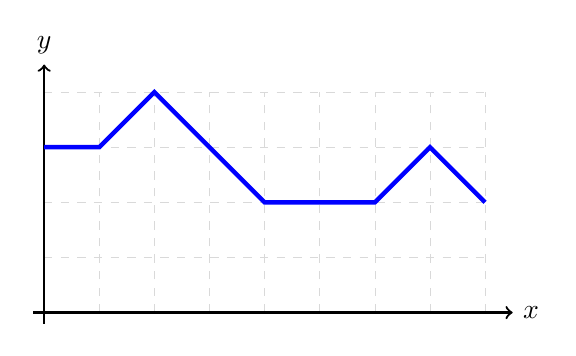
\begin{tikzpicture}[scale=0.7]
			\draw[help lines, color=gray!30, dashed] (0,0) grid (8,4);
			\draw[->,thick] (-0.2,0) -- (8.5,0) node[right] {$x$};
			\draw[->,thick] (0,-0.2) -- (0,4.5) node[above] {$y$};
			\draw[ultra thick,blue] (0,3)--++(1,0)--++(1,1)--++(2,-2)--++(2,0)--++(1,1)--++(1,-1);
		\end{tikzpicture}
	\caption{Example of a lattice path starting at height 3.}
		\label{fig:motzkin}
	\end{center}
\end{figure}

Now, each term in the sum in \eqref{eq:tridiagonal-moments-expansion}
corresponds to a path. Moreover, for each path shape,
there are $O(n)$ summands corresponding to it. The number of
paths of length $k$ starting from a fixed $m$ 
is finite (independent of $n$ for $m\gg 1$),
so we need to look more closely at the asymptotics of the product
in \eqref{eq:tridiagonal-moments-expansion}. This product
involves chi random variables which depend on $n$, too.

%%%%%%%%%%%%%%%%%%%%%%%%%%%%%%%%%%%%%%%%%%%%%%%%%%%%%%%%%%%%
\subsection{Asymptotics of chi random variables}
\label{sub:chi-asymptotics}
%%%%%%%%%%%%%%%%%%%%%%%%%%%%%%%%%%%%%%%%%%%%%%%%%%%%%%%%%%%%

One additional technical point in analyzing $T/\sqrt{n}$ is to note that $\alpha_j$
is roughly $\sqrt{\beta(n-j)/2}$ for large $n$.
Indeed, we have
\begin{equation*}
	\chi^2_\nu=\sum_{i=1}^\nu Z_i^2,\qquad
	\operatorname{\mathbb{E}}[\chi^2_\nu]=\nu,\qquad
	\operatorname{Var}[\chi^2_\nu]=2\nu.
\end{equation*}
Now, since we are dividing by $\sqrt n$, we have
\begin{equation*}
	\frac{\alpha_j}{\sqrt n}\sim \sqrt{\frac{\beta}{2}}\sqrt{1-\theta},\qquad
	\theta=\frac{j}{n}\in [0,1].
\end{equation*}
This estimate is valid in the ``bulk'' region, that is, when $\theta$ is strictly between $0$ and $1$.

Let us make these estimates more precise.  We have:
\begin{proposition}[Pointwise asymptotics in the bulk]
\label{prop:alpha-bulk}
Fix any $\delta \in (0,1)$ and let $j$ range so that $\theta_j := j/n \in [\delta,\, 1-\delta]$.
Then for each such $j$, we have\footnote{Here and below, $O_p(\cdot)$ denotes a term that is stochastically bounded at the indicated order as $n\to\infty$. That is, $X_n = O_p(a_n)$ means that for any $\epsilon>0$, there exists $M>0$ such that $\Pr(|X_n/a_n| > M) < \epsilon$ for all sufficiently large $n$.}
\[
  \frac{\alpha_j}{\sqrt{n}}
  \;=\; \sqrt{\beta\Bigl(1 - \frac{j}{n}\Bigr)}
  \;+\; O_p\Bigl(\frac{1}{\sqrt{n}}\Bigr),
\]
In particular,
\[
  \lim_{n\to\infty} \frac{\alpha_j}{\sqrt{n}}
  \;=\; \sqrt{\beta\Bigl(1-\theta_j\Bigr)}
  \quad\text{in probability.}
\]
\end{proposition}


\begin{remark}
Outside the bulk region (i.e.\ very close to $j=0$ or $j=n$), one would need a different statement to handle the case $\beta(n-j)$ is not large.
In our application, we only need the bulk behavior.
\end{remark}

Meanwhile, on the diagonal, $d_i/\sqrt{n}$
almost surely vanishes in the limit as $n\to\infty$,
because $d_i$ is standard Gaussian and does not depend on $n$.



%%%%%%%%%%%%%%%%%%%%%%%%%%%%%%%%%%%%%%%%%%%%%%%%%%%%%%%%%%%%
\subsection{Completing the proof: global semicircle behavior}
%%%%%%%%%%%%%%%%%%%%%%%%%%%%%%%%%%%%%%%%%%%%%%%%%%%%%%%%%%%%

Putting the above pieces together, we see that
\begin{equation}
	\label{eq:tridiagonal-moments-discussion}
	\frac{T}{\sqrt n}=
	\frac{1}{n}
	\sum_{i_1,\dots,i_k=1}^n
	\prod_{\ell=1}^k
	\frac{t_{i_\ell i_{\ell+1}}}{\sqrt n},\quad
	i_{k+1}=i_1 \textnormal{ by agreement}.
\end{equation}
The terms in the sum have all $i_{\ell}$'s close together
(there are $k$ indices, and they differ by $\pm1$ from each other).
We
may think that they are close to some $\theta n$, where $\theta\in [0,1]$.
We can consider only the case when $\delta<\theta<1-\delta$ for some fixed small $\delta>0$;
the case of edges does not contribute (see Problem~\ref{prob:edges-in-tridiagonal}).

If at least one of the $t_{ij}$'s in \eqref{eq:tridiagonal-moments-discussion} is
on the diagonal, the term vanishes in the limit. Therefore,
it suffices to consider only the off-diagonal $\alpha_j$'s. The
number of length $k$ walks starting from $m=\theta n$ for $\theta>\delta$ is 
just the number of lattice walks with steps $(1,\pm 1)$. This number is $\binom{k}{k/2}$.\footnote{Not Catalan yet!}
(From now on till the end of the section, we assume that
$k$ is even --- the moments become zero for odd $k$).

Fixing the starting location $\theta=\frac{i_\ell}{n}\in(\delta,1-\delta)$, we have
\begin{equation*}
	\prod_{\ell=1}^k
	\frac{t_{i_\ell i_{\ell+1}}}{\sqrt n}\to \beta^{k/2}(1-\theta)^{k/2}.
\end{equation*}

There is an extra factor $1/n$ in front in \eqref{eq:tridiagonal-moments-discussion},
which is interpreted as transforming the sum over $i_1,\ldots,i_k $
into an integral in $\theta$. We thus see that the moments converge to
\begin{equation*}
	\beta^{k/2}\binom{k}{k/2}\int_0^1 (1-\theta)^{k/2} \, d\theta=
	\beta^{k/2}\binom{k}{k/2}\cdot \frac{1}{1+k/2}, 
\end{equation*}
and we recover our favorite
Catalan moments of the semicircle distribution.

This completes the proof.

\begin{remark}[The factor $\beta^{k/2}$]
	Note that the factor $\beta^{k/2}$ refers just to the scaling of the Wigner
	semicircle law, and does not affect the semicircle shape. More precisely, 
	the limiting semicircle distribution lies from $[-2\sqrt{\beta},2\sqrt{\beta}]$.
\end{remark}

\section{Wigner semicircle law via Stieltjes transform}

Let us stay in the tridiagonal setting, and explore a more analytic
method to derive the Wigner semicircle law.



In this supplemental note, we elaborate on the \emph{Stieltjes transform} (resolvent) approach to proving the Wigner semicircle law for Gaussian and, more generally, Wigner-type matrices.  We base our discussion on a key simplification: \emph{tridiagonalization} of real symmetric matrices.  

The argument proceeds in several steps:
\begin{enumerate}[\(\bullet\)]
\item We recall from the previous lectures that any real symmetric matrix \(W\) can be conjugated by an orthogonal transformation to a real tridiagonal matrix \(T\).  For a GOE random matrix, the distribution of \(T\) is explicitly known (Dumitriu--Edelman form).
\item We rewrite spectral questions about \(W\) in terms of the (much sparser) tridiagonal matrix \(T\).  In particular, the matrix resolvent \((T - zI)^{-1}\) is easier to analyze through a recurrence relation.
\item By taking traces of the resolvent, we obtain the Stieltjes transform of the empirical eigenvalue distribution (ESD).  Its \emph{large \(n\) limit} is forced to satisfy a known algebraic equation whose unique solution is the semicircle law.
\end{enumerate}

We will thus see a more direct linear-algebraic interpretation of the random matrix’s global spectral behavior, complementing the combinatorial ``moment-counting'' method from earlier.

\section{Tridiagonal Structure and Characteristic Polynomials}
\label{sec:tridiag-charpoly}

We consider a real symmetric tridiagonal matrix 
\[
  T \;=\;
  \begin{pmatrix}
    d_1 & \alpha_1 & 0 & \cdots & 0 \\
    \alpha_1 & d_2 & \alpha_2 & \ddots & \vdots \\
    0 & \alpha_2 & d_3 & \ddots & 0 \\
    \vdots & \ddots & \ddots & \ddots & \alpha_{n-1} \\
    0 & \cdots & 0 & \alpha_{n-1} & d_n
  \end{pmatrix},
\]
of size \(n\times n\).  We let
\[
  T - \lambda I = 
  \begin{pmatrix}
    d_1 - \lambda & \alpha_1 & 0 & \cdots \\
    \alpha_1 & d_2 - \lambda & \alpha_2 & \ddots \\
    0 & \alpha_2 & d_3 - \lambda & \ddots \\
    \vdots & \ddots & \ddots & \ddots
  \end{pmatrix}.
\]
We want to understand its eigenvalues, or equivalently, its characteristic polynomial.  

\subsection{Three-Term Recurrence for the Characteristic Polynomial}

For each \(k=1,\dots,n\), denote by \(T_k\) the top-left \(k\times k\) submatrix of \(T\).  Define the \emph{characteristic polynomial} of that block:
\[
  p_k(\lambda) \;=\; \det\bigl(T_k - \lambda I_k\bigr).
\]
By convention, set \(p_0(\lambda)\coloneqq 1\).  Then a basic determinant expansion argument along the last row or column shows:

\begin{lemma}[Three-Term Recurrence]
\label{lem:3term}
For each \(k\ge1\), we have
\[
  p_{k+1}(\lambda)
  \;=\;
  (d_{k+1}-\lambda)\,p_k(\lambda)
  \;-\;\alpha_k^2\,p_{k-1}(\lambda).
\]
Equivalently, we have 
\[
  p_1(\lambda) = (d_1 - \lambda), 
  \qquad
  p_2(\lambda) = (d_2 - \lambda)\,(d_1-\lambda)\,-\,\alpha_1^2,
\]
and in general one proceeds by induction. 
\end{lemma}

Thus the characteristic polynomial \(\det(T - \lambda I)\) satisfies a simple linear recurrence in \(k\).  In orthogonal polynomial language, one may think of \(\{p_k(\lambda)\}\) as a family of monic polynomials in \(\lambda\) with a three-term recursion and certain initial conditions.

\subsection{Spectral Connection and Eigenvalues}

The eigenvalues \(\lambda_1,\dots,\lambda_n\) of \(T\) are exactly the roots of \(p_n(\lambda)\).  For any \(\lambda \in \mathbb{C}\), if \(\lambda\) is not an eigenvalue, then \(\bigl(T - \lambda I\bigr)\) is invertible.  

When \(\lambda\) is close to a real eigenvalue, the behavior of the resolvent \(\bigl(T-\lambda I\bigr)^{-1}\) becomes large.  Tracking these poles in the complex plane is the key to the resolvent or Stieltjes transform approach.

\section{Stieltjes Transform / Resolvent}
\label{sec:stieltjes-def}

Recall that for a matrix \(A\) with real eigenvalues \(\lambda_1,\dots,\lambda_n\), the \emph{Stieltjes transform} (or Green’s function, or resolvent trace) is
\[
  G_n(z)
  \;=\;
  \frac{1}{n}\,\mathrm{Tr}\bigl[(A - zI)^{-1}\bigr],
  \quad
  z\in \mathbb{C}\setminus\mathbb{R}.
\]
If \(z=x+\mathrm{i}y\) is in the upper half-plane (\(y>0\)), this $G_n(z)$ can be seen as
\[
  G_n(z) 
  \;=\;
  \int_{\mathbb{R}}\!\!\frac{d\mu_n(\lambda)}{\lambda - z},
\]
where \(\mu_n = \frac{1}{n}\sum_{k=1}^n \delta_{\lambda_k}\) is the empirical spectral measure.  Equivalently, \(\mathrm{Im}\,G_n(x+\mathrm{i}0^+)\) encodes the density of eigenvalues around \(x\).  Thus, understanding $G_n(z)$ for large $n$ pinpoints the limiting spectral distribution.

\subsection{Resolvent of a Tridiagonal Matrix: Recurrence Relations}

Let us apply this to \(A = T/\sqrt{n}\) (an $n\times n$ tridiagonal matrix).  We want 
\[
  \bigl(T/\sqrt{n} - zI\bigr)^{-1},
\]
for complex \(z\).  Since $T/\sqrt{n}$ has nonzero entries only on the main and first off-diagonals, one can write down a linear recurrence for the entries of the resolvent.  

Concretely, let us denote \(\bigl(T/\sqrt{n}-zI\bigr)^{-1} = (R_{ij})\).  Then from the definition
\[
  \bigl(T/\sqrt{n} - zI\bigr)\,(R_{ij}) 
  \;=\;
  I,
\]
one gets for each row $k$:
\[
   \frac{d_k}{\sqrt{n}}\,R_{kj}
   \;-\;z\,R_{kj}
   \;+\;
   \frac{\alpha_{k-1}}{\sqrt{n}}\,R_{k-1,j}\,\mathbf{1}_{(k>1)}
   \;+\;
   \frac{\alpha_{k}}{\sqrt{n}}\,R_{k+1,j}\,\mathbf{1}_{(k<n)}
   \;=\;\delta_{k=j}.
\]
This can be reorganized into a second-order \emph{linear difference equation} in $k$ for each fixed column index $j$.  Similarly, one obtains boundary conditions.  

Because the $\alpha_k$ and $d_k$ are random but \emph{independent and identically distributed} in a suitable sense (for the GOE or general $\beta$ tridiagonal form), the coefficients in this difference equation become “stationary” for large $n$ except near the boundaries.  In fact, up to small fluctuations, $\alpha_{k}/\sqrt{n}$ stays near $\alpha$ for some constant $\alpha$ (like $\alpha\approx 1/\sqrt{2}$ if off-diagonal variance is $\frac12$), and $d_k/\sqrt{n}\to0$ with $k$.  One can then guess that 
\[
  G_n(z) \;=\; \frac{1}{n}\sum_{k=1}^n R_{kk}
\]
has a continuum limit satisfying a certain \emph{algebraic} equation.

\section{Functional Equation for the Limit and the Semicircle Law}
\label{sec:functional-eq}

Let us sketch more precisely how $G_n(z)$ converges to the semicircle transform.  

\begin{enumerate}[(1)]
\item \textbf{Asymptotic stationarity.}  By a law of large numbers or a concentration argument on $\chi^2_{\,n-j}$ (when we do the Dumitriu--Edelman version), the subdiagonal $\alpha_j$ is close to $\sqrt{(n-j)/2}$, hence $\alpha_j/\sqrt{n}\approx \sqrt{\frac{1-j/n}{2}}$.  In the bulk of the index range (where $j\approx \theta n$ for some $\theta\in(0,1)$), this is about $\sqrt{\tfrac{1-\theta}{2}}$.  Meanwhile $d_i/\sqrt{n}\approx 0$.  

\item \textbf{Discrete difference to continuous ODE.}  The second-order difference equation for $R_{k+1,k\pm1}$ is roughly
\[
  -z\,R_{k,j} \;+\; \bigl(\alpha_k/\sqrt{n}\bigr)\,R_{k+1,j}
         \;+\;\bigl(\alpha_{k-1}/\sqrt{n}\bigr)\,R_{k-1,j}
  \;=\; \delta_{k=j},
\]
neglecting the small diagonal $d_k/\sqrt{n}$ term.  In the limit $n\to\infty$, if we interpret $k/n$ as $x\in[0,1]$, then $R_{k\pm1,j}$ becomes $R(x\pm \tfrac1n)$, and $\alpha_{k}/\sqrt{n}\approx \alpha(x)$ for some function $\alpha$.  This difference equation becomes an approximate differential equation in $x$, from which one solves for $R(x,\theta)$ (thinking of $j$ as $\theta n$).  

\item \textbf{Solving for $G(z)$.}  Summing $R_{k,k}$ over $k$ becomes an integral of $R(x,x)$ over $x\in[0,1]$.  One obtains an algebraic equation in $G(z)$ akin to
\[
  G(z)^2 + z\,G(z) + 1 = 0.
\]
(Here we used normalizations that match the classical semicircle radius 2 or $\pm\sqrt{z^2-4}$ form.)  Solving for $G(z)$, we get
\[
   G(z) \;=\; \frac{-z \pm \sqrt{z^2 - 4}}{2},
\]
and the negative branch is selected by the imaginary part condition (i.e.\ $G(z)\sim -1/z$ for large $|z|$).  

\item \textbf{Back to the real axis.}  From $G(z)$ in the upper half-plane, one extracts the limit distribution by looking at $\mathrm{Im}\,(G(x+\mathrm{i}0^+))$ for real $x$.  The square-root $\sqrt{x^2-4}$ is purely imaginary for $|x|<2$, giving the semicircle density on $[-2,2]$.  

\end{enumerate}

Thus, in the limit, the spectral measure is forced to match the one whose Stieltjes transform is $G(z)$.  Since that is exactly the Wigner semicircle distribution, we conclude:

\begin{theorem}[Semicircle Law via Resolvent]
\label{thm:stieltjes-semicircle}
Let $T$ be the Dumitriu--Edelman G$\beta$E tridiagonal matrix (in particular, the GOE case when $\beta=1$) with diagonal $d_i/\sqrt{n}$ and subdiagonals $\alpha_j/\sqrt{n}$.  Then as $n\to\infty$, its empirical spectral distribution converges weakly (almost surely) to the Wigner semicircle law on $[-2,2]$.  Equivalently, its Stieltjes transform $G_n(z)$ converges for each $z\in\mathbb{C}^+$ to the unique solution of $G(z)^2 + zG(z) + 1=0$, which yields the semicircle density.
\end{theorem}

\begin{remark}
One can make this rigorous by carefully bounding the difference between $(\alpha_j/\sqrt{n})$ and its limiting profile, as well as controlling the diagonal $(d_i/\sqrt{n})$.  The approach is an archetype for many \emph{local laws} in random matrix theory, where one obtains more precise estimates on the resolvent entries for $z$ in small neighborhoods near the real axis \cite{erdHos2017dynamical,tao2012topics}.
\end{remark}

\section{Concluding Remarks}

We have now seen \emph{two main proof strategies} for deriving the Wigner semicircle law:

\begin{enumerate}[\(\bullet\)]
\item \textbf{Moment expansions and Catalan counting}: Expand $\operatorname{Tr}((W/\sqrt{n})^k)$, interpret it as a sum over closed walks, identify the main combinatorial configurations, show that the expected moments converge to the Catalan numbers that match the semicircle distribution.

\item \textbf{Stieltjes transform and resolvent analysis}: Tridiagonalize $W$, then exploit the near one-dimensional recurrence for the inverse $(T/\sqrt{n}-zI)^{-1}$.  In the large-$n$ limit, show that $G_n(z)$ satisfies a deterministic algebraic equation forcing the semicircle $G(z)$.

\end{enumerate}

Both lead to the same final statement of the global spectral distribution being the semicircle law.  The resolvent method paves the way for refined \emph{local} analysis (spectrum on small intervals) and \emph{universality proofs}.




\section{Determinantal point processes}
\label{sec:determinantal}

We are now going to start the discussion of the local eigenvalue 
behavior at $\beta=2$, started in \Cref{subsec:beta2-case}.



\appendix
\setcounter{section}{3}

\section{Problems (due 2025-02-28)}

\subsection{Eigenvalue density of G$\beta$E}

Read and understand the main principles of the
proof of \Cref{thm:DE-joint-eigenvalue-density}
in \cite{dumitriu2002matrix}.

\subsection{Chi-square mean and variance}

Let $X$ be a random variable with $\chi^2_\nu$ distribution. Compute the mean and variance of $X$.
(If $\nu$ is an integer, you can use the fact that $\chi^2_\nu$ is a sum of $\nu$ independent squares of standard normal random variables.
How to extend this to non-integer \(\nu\)?)

\subsection{Edge contributions in the tridiagonal moment computation}
\label{prob:edges-in-tridiagonal}

Show that the cases when the $i_{\ell}$'s are close to the edge ($\theta=0$ or $1$)
in \eqref{eq:tridiagonal-moments-discussion}
do not contribute to the limit of the moments.





\bibliographystyle{alpha}
\bibliography{bib}


\medskip

\textsc{L. Petrov, University of Virginia, Department of Mathematics, 141 Cabell Drive, Kerchof Hall, P.O. Box 400137, Charlottesville, VA 22904, USA}

E-mail: \texttt{lenia.petrov@gmail.com}


\end{document}
